\chapter{RV12 Execution Pipeline}

The RV12 implements a 32/64bit Integer modified form of the classic RISC pipeline. 
The pipeline consists of the Instruction Fetch, Pre-Decode, Instruction Decode, Execution, and Write Back stages as highlighted in the figure below.
 

\begin{figure}[h]
  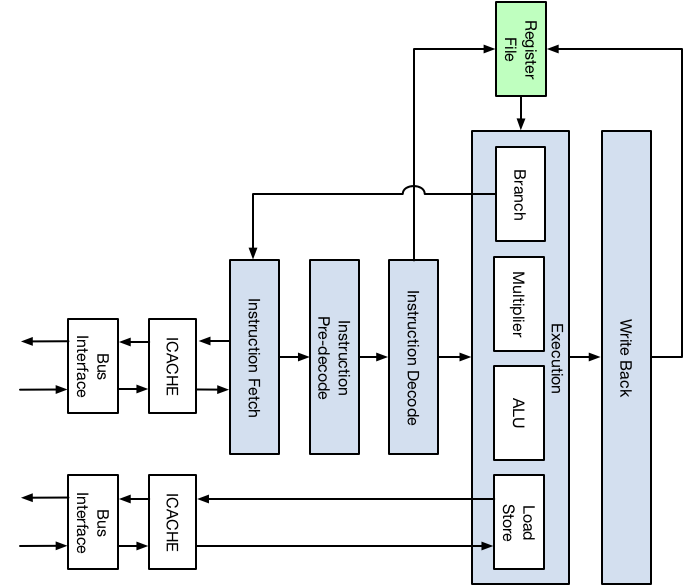
\includegraphics{assets/img/Pipeline-Overview}
  \caption{RV12 Execution Pipeline}
\end{figure}

\pagebreak

\section{Instruction Fetch (IF)}\label{instruction-fetch-if}

\begin{figure}[h]
  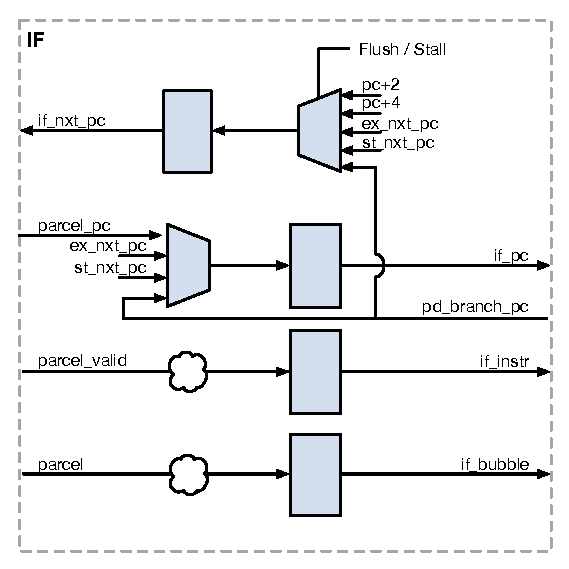
\includegraphics{assets/img/Pipeline-IF}
  \caption{Instruction Fetch Stage Implementation}
\end{figure}

The Instruction Fetch unit loads a new parcel from the program memory.
A parcel is a code field that contains one or more instructions. 
The address of the parcel to load is held by the Program Counter (PC). 
The Program Counter is either 32 or 64bits wide, depending on the XLEN parameter. 
The Program Counter is updated whenever the Instruction Pipeline is not stalled.

In case the pipeline must be flushed the Program Counter is restarted from the given address.

\begin{longtable}[]{@{}lccl@{}}
	\toprule
	\textbf{Signal} & \textbf{Direction} & \textbf{To/From} & \textbf{Description}\tabularnewline
	\midrule

	\endhead


	\texttt{if\_nxt\_pc}    & to   & Bus Interface & Next address to fetch parcel from\\
	\texttt{parcel\_pc}     & from & Bus Interface & Fetch parcel's address\\
	\texttt{parcel\_valid}  & from & Bus Interface & Valid indicators for parcel\\
	\texttt{parcel}         & from & Bus Interface & Fetched parcel\\
	& & &\\
	\texttt{Flush}          & from & EX/State      & When asserted flushes the pipe\\
	\texttt{Stall}          & from & PD            & When asserted stalls the pipe\\
	\texttt{pd\_branch\_pc} & from & PD            & New program counter for a branch instruction\\
	\texttt{if\_pc}         & to   & PD            & Instruction Fetch program counter\\
	\texttt{if\_instr}      & to   & PD            & Instruction Fetch instruction\\
	\texttt{if\_bubble}     & to   & PD            & Instruction Fetch bubble\\
		
	\bottomrule
\caption{IF Signals}
\label{tab:if-signals}
\end{longtable}

\pagebreak

\section{Pre-Decode (PD)}\label{pre-decode-pd}

The Pre-Decode unti translates 16-bit compressed instructions to the base 32bit RISC-V instructions and then processes Program Counter modifying instructions. 
Jump-And-Link and Branch instructions modify the Program Counter in the Instruction Fetch stage. 
This avoids waiting for the Execution stage to trigger the update and reduces the demand for pipeline flushes.
The destination address for branches is predicted based on the data provided by the optional Branch Prediction Unit or determined statically based on the offset.


\begin{figure}[th]
  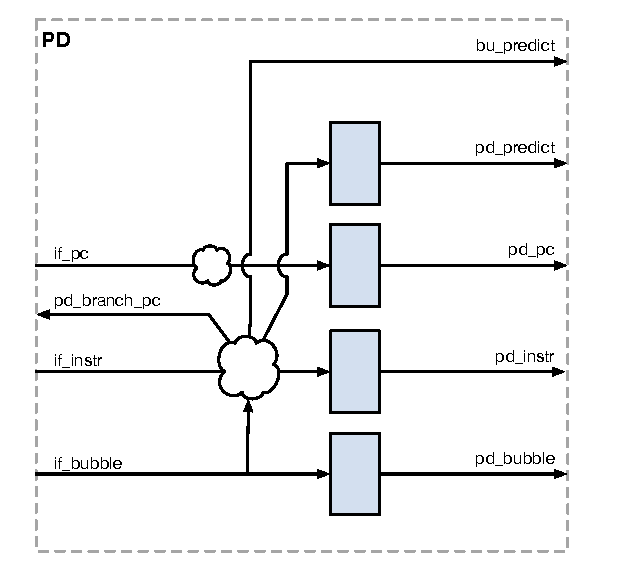
\includegraphics{assets/img/Pipeline-PD}
  \caption{Instruction Pre-Decode Stage}
\end{figure}

\begin{longtable}[]{@{}lccl@{}}
	\toprule
	\textbf{Signal} & \textbf{Direction} & \textbf{To/From} & \textbf{Description}\tabularnewline
	\midrule

	\endhead
	
	\texttt{if\_pc}         & from & IF & Instruction\_fetch program counter\\
	\texttt{if\_instr}      & from & IF & Instruction\_fetch instruction\\
	\texttt{if\_bubble}     & from & IF & Instruction\_fetch bubble\\
	\texttt{pd\_branch\_pc} & to   & IF & New PC (for a branch instruction)\\
	& & &\\
	\texttt{bu\_predict}    & from & BP & Branch prediction from Branch Prediction Unit\\
	\texttt{pd\_predict }   & to   & ID & Forwarded branch prediction\\
	\texttt{pd\_pc}         & to   & ID & Pre-Decode program counter\\
	\texttt{pd\_instr}      & to   & ID & Pre-Decode instruction\\
	\texttt{pd\_bubble}     & to   & ID & Pre-Decode bubble\\
	\bottomrule
	\caption{PD Signals}
	\label{tab:pd-signals}
\end{longtable}

\pagebreak

\section{Instruction Decode (ID)}\label{instruction-decode-id-1}

The Instruction Decode unit ensures the operands for the execution units are available. 
It accesses the Register File, calculates immediate values, and sets bypasses.

\begin{figure}[h]
  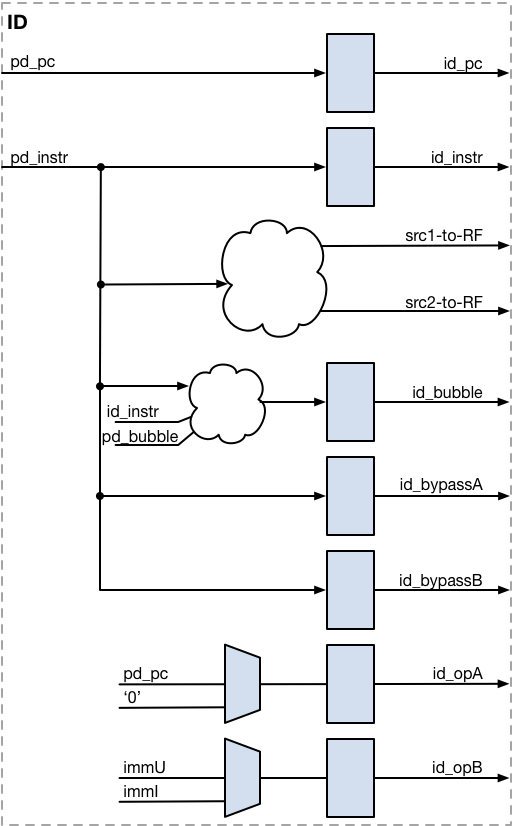
\includegraphics{assets/img/Pipeline-ID}
  \caption{Instruction Decode Stage Implementation}
\end{figure}

\begin{longtable}[]{@{}lccl@{}}
	\toprule
	\textbf{Signal} & \textbf{Direction} & \textbf{To/From} & \textbf{Description}\tabularnewline
	\midrule

	\endhead
	
		\texttt{pd\_pc}	     & from & PD & Pre-Decode program counter\\
		\texttt{pd\_instr}   & from & PD & Pre-Decode instruction\\
		\texttt{pd\_bubble}  & from & PD & Pre-Decode bubble\\
		& & &\\
		\texttt{src1}        & to   & RF & Source Register1 index\\
		\texttt{src2}        & to   & RF & Source Register2 Index\\
		& & &\\			
		\texttt{id\_bypassA} & to   & EX & Bypass signals for srcA\\
		\texttt{id\_bypassB} & to   & EX & Bypass signals for srcB\\
		\texttt{id\_opA}     & to   & EX & Calculated operandA\\
		\texttt{id\_opB}     & to   & EX & Calculated operandB\\
		\texttt{id\_pc}      & to   & EX & Instruction Decode program counter\\
		\texttt{id\_instr}   & to   & EX & Instruction Decode instruction\\
		\texttt{id\_bubble}  & to   & EX & Instruction Decode bubble\\	
	\bottomrule
	\caption{ID Signals}
	\label{tab:id-signals}
\end{longtable}

\pagebreak

\section{Execute (EX)}\label{execute-ex-1}

The Execute stage performs the required operation on the data provided by the Instruction Decode stage. 
The Execution stage has multiple execution units, each with a unique function.
The ALU performs logical and arithmetic operations.
The Multiplier unit calculates signed/unsigned multiplications.
The Divider unit calculates signed/unsigned division and remainder.
The Load-Store Unit accesses the data memory.
The Branch Unit calculates jump and branch addresses and validates the predicted branches.

Only one operation can be executed per clock cycle.
Most operations complete in one clock cycle, except for the divide instructions, which always take multiple clock cycles to complete. 
The multiplier supports configurable latencies, to improve performance.


\begin{figure}[h]
  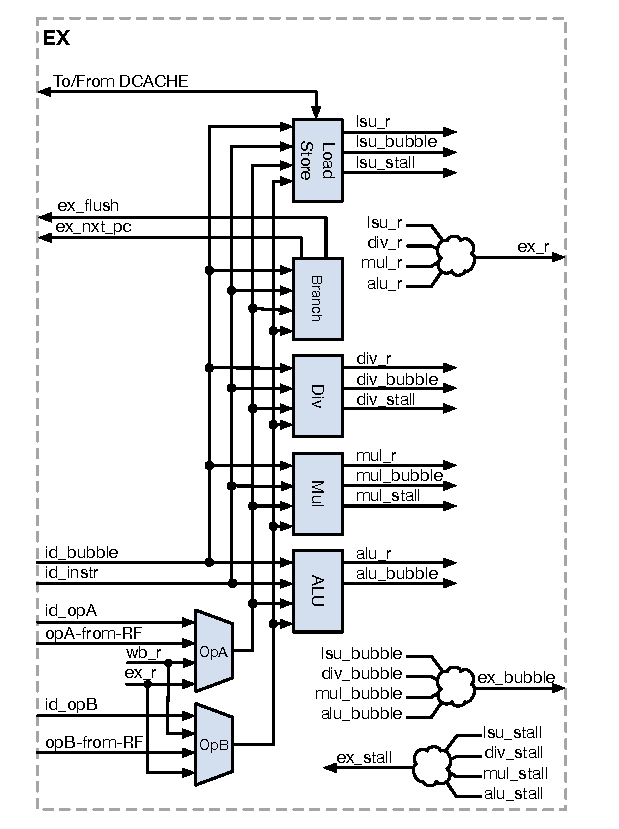
\includegraphics{assets/img/Pipeline-EX}
  \caption{Execute Stage Implementation}
\end{figure}

\begin{longtable}[]{@{}lccl@{}}
	\toprule
	\textbf{Signal} & \textbf{Direction} & \textbf{To/From} & \textbf{Description}\tabularnewline
	\midrule

	\endhead
		id\_pc      & from & ID       & Instruction Decode program counter\\
		id\_instr   & from & ID       & Instruction Decode instruction\\
		id\_bubble  & from & ID       & Instruction Decode bubble\\
		            &      &          & \\
		opA         & from & RF       & Source Register1 value\\
		opB         & from & RF       & Source Register2 value\\
		            &      &          & \\
		id\_bypassA & from & ID       & Bypass signals for srcA\\
		id\_bypassB & from & ID       & Bypass signals for srcB\\
		id\_opA     & from & ID       & Calculated operandA\\
		id\_opB     & from & ID       & Calculated operandB\\
		ex\_stall   & to   & ID       & Stall ID (and higher) stages\\
		ex\_flush   & to   & ID/PD/IF & Flush ID (and higher) pipe stages\\
		ex\_r       & to   & WB       & Result from execution units\\
		ex\_pc      & to   & WB       & Execute program counter\\
		ex\_instr   & to   & WB       & Execute instruction\\
		ex\_bubble  & to   & WB       & Execute bubble\\
	\bottomrule
	\caption{EX Signals}
	\label{tab:ex-signals}
\end{longtable}

\pagebreak

\section{Write-Back (WB)}\label{write-back-wb-1}

The Write-Back stage writes the results from the Execution Unit into the Register File.

\begin{figure}[h]
  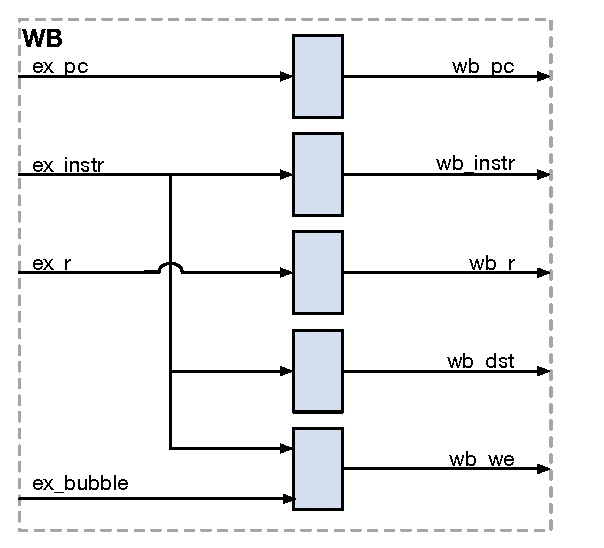
\includegraphics{assets/img/Pipeline-WB}
  \caption{Write-back Stage Implementation}
\end{figure}

\begin{longtable}[]{@{}lccl@{}}
	\toprule
	\textbf{Signal} & \textbf{Direction} & \textbf{To/From} & \textbf{Description}\tabularnewline
	\midrule
	\endhead
		\texttt{ex\_pc}     & from & EX & Execute program counter\\
		\texttt{ex\_instr}  & from & EX & Execute instruction\\
		\texttt{ex\_bubble} & from & EX & Execute bubble\\
		\texttt{ex\_r}      & from & EX & Result from execution units\\
		                    &      &    & \\
		\texttt{wb\_r}      & to   & RF & Result to be written to RF\\
		\texttt{wb\_dst}    & to   & RF & Destination register index\\
		\texttt{wb\_we}     & to   & RF & Write enable\\
		\texttt{wb\_pc}     & to   & WB & WriteBack program counter\\
		\texttt{wb\_instr}  & to   & WB & WriteBack instruction\\

	\bottomrule
	\caption{EWBSignals}
	\label{tab:wb-signals}
\end{longtable}


